    \documentclass[a4]{article}

    % PAQUETES %%%%%%%%%%%%%%%%%%%%%%%%%%%%%%%%%%%%%%%%%%%%%%%%%%%%%%%%%%%%%%%%%%%%%
    \usepackage[utf8]{inputenc}
    \usepackage{framed} % Para crear cuadros alrededor del texto
    \usepackage{makecell}
    \usepackage[english]{babel}
    %
    \usepackage{comment}
    \usepackage[fixlanguage]{babelbib}
        \bibliographystyle{IEEEtran}

    \usepackage{url}

    %!TEX encoding = UTF-8 Unicode
    % !TEX spellcheck = es

    \setlength{\textwidth}{6.5 in}
    \setlength{\textheight}{8.5 in}
    \setlength{\headsep}{0.5 in}

    \usepackage{multirow, array} % para las tablas
    \usepackage{float} % para usar [H]
    \usepackage{charter}

    \usepackage[breaklinks=true]{hyperref}

    %
    % ADD PACKAGES here:
    %

    \usepackage[utf8]{inputenc}
    \usepackage{amsmath,longtable,siunitx, float, graphicx, dcolumn, bm, fancyhdr, authblk, subcaption, caption, hyperref, multicol, setspace}

    \usepackage{bbding}
    \usepackage{amssymb}
    \usepackage[rightcaption]{sidecap}
    %\usepackage{textcomp}

    \usepackage[hmarginratio=1:1, top=32mm, columnsep=20pt, headsep=\dimexpr20mm, margin=0.7in, top=1in ]{geometry}

    \usepackage{booktabs}
    \usepackage{multirow}

    \usepackage{algorithm}
    \usepackage{enumitem}
    \usepackage{tabularx}
    \usepackage[noend]{algpseudocode}
    \usepackage{xcolor}

    \usepackage{tikz}
    \usetikzlibrary{shapes.geometric, arrows.meta, positioning}

    % ----------- global styles -----------
    \tikzset{
      font=\scriptsize,                      % tiny text everywhere
      every node/.style       = {transform shape},   % respect scale
      startstop/.style        = {ellipse, draw, fill=blue!10,
                                 inner sep=1pt, minimum width=13mm},
      process/.style          = {rectangle, draw, fill=orange!15,
                                 text width=26mm, inner sep=2pt, align=center},
      decision/.style         = {diamond, draw, fill=green!15, aspect=2.3,
                                 text width=20mm, inner sep=1pt, align=center},
      arrow/.style            = {->, >=Stealth, shorten >=1pt, shorten <=1pt}
    }

    \newcommand{\TODO}{\textbf{\textcolor{red}{TODO}}}

    \renewcommand{\algorithmicrequire}{\textbf{Input:}}
    \renewcommand{\algorithmicensure}{\textbf{Output:}}

    \lhead{\includegraphics[scale=0.4]{CETC.png}}
    \rhead{\includegraphics[scale=0.025]{Cornell-University-Logo.png}}

    \newtheorem{theo}{Theorem}
    \newenvironment{theorem}
      {\begin{mdframed}\begin{theo}}
      {\end{theo}\end{mdframed}}

    \newtheorem{prop}{Proposición}
    \newenvironment{proposition}
      {\begin{mdframed}\begin{prop}}
      {\end{prop}\end{mdframed}}

    \newtheorem{lem}{Lema}
    \newenvironment{lema}
      {\begin{mdframed}\begin{lem}}
      {\end{lem}\end{mdframed}}

    \newtheorem{defi}{Definition}
    \newenvironment{definition}
      {\begin{mdframed}\begin{def}}
      {\end{def}\end{mdframed}}

    \newtheorem{proof}{Proof}
    \newtheorem{remark}{Remark}

    \usepackage[numbers]{natbib}
    \renewcommand{\thesection}{\Roman{section}}
    %\setlength{\parskip}{\baselineskip}%

\begin{document}

\thispagestyle{fancy}

\begin{center}
    \textbf{\Large Orbit Odyssey --- Computer Vision} \\[4pt]
    {\large Complete Competition Manual}

    \vspace{0.7em}

    David Alejandro Fuquen \\

    {\small \today}

\end{center}

%=============================================================================
\section{Introduction \& Mission}
%=============================================================================

Welcome to the Orbit Odyssey Computer Vision Challenge! Two teams compete simultaneously on a shared arena, each training an object detection model, deploying it on an Intel AIxBoard, and letting an XRP robot act \textbf{autonomously} based on what it sees through its camera. You will not control the robot during the challenge: your model and your code determine how well the robot performs.

This manual covers everything in one place: the arena layout, object behaviors, competition rules, scoring, model training, competition day procedures, moderator instructions, and a printable scorecard.

\subsection*{The Mission}

The year is 2147. A cargo shuttle carrying critical supplies has crash-landed on the surface of a remote moon. The impact scattered debris across the crash site, and several \textbf{escape pods} were ejected on impact and now lie among the wreckage. Two rival engineering teams have each been tasked with deploying an autonomous rescue rover to opposite halves of the crash site.

Your rover must navigate the debris field:
\begin{itemize}
    \item \textbf{Contact each escape pod} (Rocket): approach it, make physical contact to activate its homing beacon, then spin clockwise and continue the search.
    \item \textbf{Avoid hazardous debris}: some wreckage is unstable.
    \begin{itemize}
        \item \textbf{Tire debris} must be avoided by spinning \textbf{clockwise}.
        \item \textbf{Tin Can debris} must be avoided by performing an \textbf{evasive maneuver}: a brief counter-clockwise feint (20\textdegree) followed by a clockwise sweep (60\textdegree).
    \end{itemize}
    \item Touching any debris triggers a containment breach.
\end{itemize}

The crash site is divided by a partition wall. Each team operates on one half. There is a catch: the rover's communication window lasts only \textbf{120 seconds}. After that, the signal is lost and the mission ends. Your team's only decision is which direction the rover faces at deployment. From that moment on, the rover must rely entirely on its camera and your trained model to identify objects and decide what to do.

The better your model, and the smarter your code, the better the rover performs.

\pagebreak
%=============================================================================
\section{The Arena}
%=============================================================================
\subsection*{Field dimensions}

The playing field is a rectangular arena enclosed by low-profile PVC pipe barriers on all four sides, with a central partition dividing it into two halves. This is the exact same field used in the original Orbit Odyssey challenge. 

\begin{table}[H]
\centering
\begin{tabular}{ll}
\toprule
\textbf{Property} & \textbf{Value} \\
\midrule
Total length (X-axis) & 254.00 cm (100 in) \\
Total width (Y-axis) & 142.24 cm (56 in) \\
Total floor area & 3.61 m\textsuperscript{2} \\
Perimeter walls & Low-profile PVC pipe barriers \\
Corner zones & 30.48 $\times$ 30.48 cm (12 $\times$ 12 in) at each corner \\
\bottomrule
\end{tabular}
\caption{Field dimensions and boundaries.}
\end{table}

The coordinate system places the origin $(0, 0)$ at the bottom-left corner of the field. The X-axis runs left to right (0 to 254 cm) and the Y-axis runs bottom to top (0 to 142.24 cm). The partition does \textbf{not} block the camera's line of sight (the camera sits above pipe height). It blocks the robot's driving path through the center 50 inches, confining each team's robot to its own half.

\subsection*{Mirrored layout}

Both teams use the same triangle arrangement, mirrored across the partition. Team~A plays in the \textbf{bottom half}; Team~B plays in the \textbf{top half}. Each half contains 3 objects and one robot starting position.

\begin{figure}[H]
\centering
\begin{tikzpicture}
  \begin{scope}[scale=0.055]
    % Field outline
    \draw[thick] (0,0) rectangle (254, 142.24);
    % Corner zones
    \draw[dashed, blue!60] (0,0) rectangle (30.48, 30.48);
    \draw[dashed, blue!60] (254-30.48,0) rectangle (254, 30.48);
    \draw[dashed, blue!60] (0,142.24-30.48) rectangle (30.48, 142.24);
    \draw[dashed, blue!60] (254-30.48,142.24-30.48) rectangle (254, 142.24);
    % Partition
    \draw[very thick, orange!80!black] (63.50, 71.12) -- (190.50, 71.12);
    % Bottom half objects (Team A) - red
    \filldraw[red!70!black] (50.80, 20.32) circle (6);
    \filldraw[red!70!black] (203.20, 20.32) circle (6);
    \filldraw[red!70!black] (127.00, 50.80) circle (6);
    % Bottom half robot
    \filldraw[green!60!black] (127.00, 30.48) circle (5);
    % Bottom triangle pattern
    \draw[dashed, gray!50] (50.80,20.32) -- (203.20,20.32) -- (127.00,50.80) -- cycle;
    % Top half objects (Team B) - blue
    \filldraw[blue!70!black] (50.80, 121.92) circle (6);
    \filldraw[blue!70!black] (203.20, 121.92) circle (6);
    \filldraw[blue!70!black] (127.00, 91.44) circle (6);
    % Top half robot
    \filldraw[green!60!black] (127.00, 111.76) circle (5);
    % Top triangle pattern
    \draw[dashed, gray!50] (50.80,121.92) -- (203.20,121.92) -- (127.00,91.44) -- cycle;
    % Dimension arrows
    \draw[<->, >=Stealth] (0,-12) -- (254,-12);
    \draw[<->, >=Stealth] (-12,0) -- (-12,142.24);
  \end{scope}
  % Bottom half labels
  \node[font=\footnotesize\bfseries, red!70!black, anchor=east] at (2.47,1.12) {\textsf{P1}};
  \node[font=\footnotesize\bfseries, red!70!black, anchor=west] at (11.51,1.12) {\textsf{P2}};
  \node[font=\footnotesize\bfseries, red!70!black, anchor=south] at (6.99,3.13) {\textsf{P3}};
  \node[font=\footnotesize\bfseries, green!40!black, anchor=west] at (7.30,1.68) {\textsf{Robot A}};
  % Top half labels
  \node[font=\footnotesize\bfseries, blue!70!black, anchor=east] at (2.47,6.71) {\textsf{P1'}};
  \node[font=\footnotesize\bfseries, blue!70!black, anchor=west] at (11.51,6.71) {\textsf{P2'}};
  \node[font=\footnotesize\bfseries, blue!70!black, anchor=north] at (6.99,4.73) {\textsf{P3'}};
  \node[font=\footnotesize\bfseries, green!40!black, anchor=west] at (7.30,6.15) {\textsf{Robot B}};
  % Partition label
  \node[font=\scriptsize, orange!80!black, anchor=south] at (6.99,4.10) {Partition};
  % Half labels
  \node[font=\footnotesize, gray] at (6.99,2.20) {Team A Half (Bottom)};
  \node[font=\footnotesize, gray] at (6.99,5.62) {Team B Half (Top)};
  % Corner zone labels
  \node[blue!70, font=\scriptsize] at (0.84,0.84) {LRZ};
  \node[blue!70, font=\scriptsize] at (13.13,0.84) {LRZ};
  \node[blue!70, font=\scriptsize] at (0.84,6.98) {LRZ};
  \node[blue!70, font=\scriptsize] at (13.13,6.98) {LRZ};
  % Dimension labels
  \node[font=\footnotesize] at (6.99,-1.10) {254 cm (100 in)};
  \node[font=\footnotesize, rotate=90] at (-1.21,3.91) {142.24 cm (56 in)};
  \node[font=\scriptsize, anchor=north east] at (-0.11,-0.11) {$(0,0)$};
\end{tikzpicture}
\caption{Mirrored P\_3 layout --- each team has 3 objects in its half.}
\end{figure}

\subsection*{Object positions}

\begin{table}[H]
\centering
\begin{tabular}{clccccc}
\toprule
\textbf{ID} & \textbf{Location} & \textbf{X (in)} & \textbf{Y (in)} & \textbf{X (cm)} & \textbf{Y (cm)} & \textbf{Half} \\
\midrule
P1 & Lower-left & 20 & 8 & 50.80 & 20.32 & Bottom \\
P2 & Lower-right & 80 & 8 & 203.20 & 20.32 & Bottom \\
P3 & Above center & 50 & 20 & 127.00 & 50.80 & Bottom \\
\midrule
P1' & Upper-left & 20 & 48 & 50.80 & 121.92 & Top \\
P2' & Upper-right & 80 & 48 & 203.20 & 121.92 & Top \\
P3' & Below center & 50 & 36 & 127.00 & 91.44 & Top \\
\bottomrule
\end{tabular}
\caption{Object positions for both halves.}
\end{table}

\begin{table}[H]
\centering
\begin{tabular}{clcc}
\toprule
\textbf{Robot} & \textbf{Location} & \textbf{Position (cm)} & \textbf{Position (in)} \\
\midrule
Robot A & Bottom half, center of triangle & (127.00, 30.48) & (50, 12) \\
Robot B & Top half, center of triangle & (127.00, 111.76) & (50, 44) \\
\bottomrule
\end{tabular}
\caption{Robot starting positions.}
\end{table}

\subsection*{Distance from robot to each object}

\begin{table}[H]
\centering
\begin{tabular}{ccc}
\toprule
\textbf{ID} & \textbf{Distance to robot (cm)} & \textbf{Distance to robot (in)} \\
\midrule
P1 (or P1') & 76.9 & 30.3 \\
P2 (or P2') & 76.9 & 30.3 \\
P3 (or P3') & 20.3 & 8.0 \\
\bottomrule
\end{tabular}
\caption{Distance from robot center to each object (identical for both halves due to symmetry).}
\end{table}

\subsection*{Clearance verification}

\textbf{Minimum clearances:} object center to wall $\geq$ 20 cm, object center to partition $\geq$ 20 cm, object center to object center $\geq$ 35 cm, objects must be outside all corner zones.

\begin{table}[H]
\centering
\begin{tabular}{ccccccc}
\toprule
\textbf{ID} & \textbf{Left wall} & \textbf{Right wall} & \textbf{Outer wall} & \textbf{Partition} & \textbf{Min wall} & \textbf{Nearest obj.} \\
\midrule
P1 & 50.8 & 203.2 & 20.3 & 50.8 \checkmark & 20.3 \checkmark & 82.1 (P3) \checkmark \\
P2 & 203.2 & 50.8 & 20.3 & 50.8 \checkmark & 20.3 \checkmark & 82.1 (P3) \checkmark \\
P3 & 127.0 & 127.0 & 50.8 & 20.3 \checkmark & 20.3 \checkmark & 82.1 (P1) \checkmark \\
\bottomrule
\end{tabular}
\caption{Clearance verification (all values in cm). Identical for both halves by symmetry.}
\end{table}

\subsection*{Class rotation templates}

Object positions are physically fixed. Between rounds, the referee assigns classes to positions using one of these templates. Both halves use the same template simultaneously.

\begin{table}[H]
\centering
\begin{tabular}{lccc}
\toprule
\textbf{Template} & \textbf{P1 / P1'} & \textbf{P2 / P2'} & \textbf{P3 / P3'} \\
\midrule
A & Rocket & Tire & Tin Can \\
B & Tin Can & Rocket & Tire \\
C & Tire & Tin Can & Rocket \\
\bottomrule
\end{tabular}
\caption{Class rotation templates. Each template ensures all 3 classes are present.}
\end{table}

\subsection*{Navigation notes}

\begin{itemize}
    \item Each team's robot operates entirely within its own half. The partition physically prevents crossing.
    \item The robot starts at the centroid of the triangle. P3 (or P3') is closest ($\sim$20 cm), directly above (or below). P1 and P2 are $\sim$77 cm away, near the left and right walls.
    \item The robot can reach any object by spinning to face it and driving forward.
\end{itemize}

\pagebreak
%=============================================================================
\section{The Objects \& Robot Behaviors}
%=============================================================================

There are three object classes. Each is a 3D-printed object with an approximate radius of 6 cm.

\subsection*{Object behaviors and scoring}

\begin{table}[H]
\centering
\begin{tabular}{llp{6.5cm}c}
\toprule
\textbf{Object} & \textbf{Type} & \textbf{Correct Robot Action} & \textbf{Points} \\
\midrule
\textbf{Rocket} & Contact & Approach, touch object, spin \textbf{clockwise} & $+20$ \\
\textbf{Rocket} & Contact (no touch) & Approach, spin \textbf{clockwise} (without touching) & $+15$ \\
\textbf{Tire} & Avoid & Approach, spin \textbf{clockwise}, drive away (no touch) & $+15$ \\
\textbf{Tin Can} & Avoid & Approach, spin \textbf{CCW 20\textdegree} then \textbf{CW 60\textdegree}, drive away (no touch) & $+15$ \\
\bottomrule
\end{tabular}
\caption{Object classes and correct robot actions.}
\end{table}

\subsubsection*{Tin Can compound rotation}

The Tin Can avoidance requires a \textbf{two-part rotation}:
\begin{enumerate}
    \item Robot approaches the Tin Can to $\sim$20 cm.
    \item Robot spins \textbf{counter-clockwise 20\textdegree} (a brief feint).
    \item Robot then spins \textbf{clockwise 60\textdegree} (the main evasion).
    \item Robot drives away without touching the object.
\end{enumerate}
The net result is approximately 40\textdegree{} clockwise. The referee must observe \textbf{both} rotation phases for the engagement to score as a correct avoid (+15). If the robot performs only a clockwise spin (missing the initial counter-clockwise feint) or any other pattern, it is scored as a wrong-direction avoid (+5).

\begin{framed}
\textbf{The Approach Requirement}

For \textbf{any} engagement to count---contact, approach, or avoid---the robot must \textbf{visibly drive toward the object} and reach approximately \textbf{20 cm or closer} before executing any spin or contact action.

\textbf{Random spinning does not count.} If the robot rotates in place near an object without first making a clear, deliberate approach, the referee will \textbf{not} score that engagement. The referee must observe a distinct forward movement toward the target object before any rotational action is performed.

This rule prevents uncontrolled spinning from being mistaken for intentional behavior. The robot must demonstrate that it \textit{recognized} the object and \textit{chose} to interact with it.
\end{framed}

\subsection*{First recognition only}

Each object is scored \textbf{exactly once}: the first time the robot engages it. Maximum \textbf{3 scored engagements} per run (one per object). Subsequent interactions with the same object are ignored for scoring purposes.

\subsection*{Misclassification consequences}

If the model \textit{misclassifies} an object (for example, labels a Tire as a Tin Can) the robot will perform the wrong rotation. This earns partial credit ($+5$, wrong-direction avoid) but costs the full $+15$.

If the robot physically \textit{touches} an avoid object, that is a \textbf{false contact} ($-10$) and also disqualifies the team from the \textbf{Clean Avoid bonus} ($+15$). A single false contact represents a net swing of $-25$ points compared to a correct avoid.

\pagebreak
%=============================================================================
\section{Rules of the Game}
%=============================================================================

\begin{enumerate}[label=\textbf{R\arabic*.}, leftmargin=2.5em]

\item \textbf{Game duration.} Each run lasts exactly \textbf{120 seconds}. Two teams play simultaneously, one in each half of the field. The timer starts on the referee's signal and never pauses. When the buzzer sounds, the run is over.

\item \textbf{Starting position.} Each robot is placed at its designated starting position: \textbf{Team A at (127.00, 30.48) cm} in the bottom half, \textbf{Team B at (127.00, 111.76) cm} in the top half. The robot starts at the centroid of its object triangle.

\item \textbf{Initial heading.} The team selects the direction the camera faces at the start. This is the \textbf{only human decision} permitted during the challenge.

\item \textbf{Hands-off rule.} From the start signal to the buzzer, \textbf{no team member may touch the robot, any object, the field surface, or the field walls} for any reason. There are no exceptions. Any unauthorized touch \textbf{immediately terminates} the run for that team, with the score recorded up to that point.

\item \textbf{Code modification.} Teams \textbf{may modify} both \texttt{main.py} (robot behavior, MicroPython) and \texttt{run\_model.py} (inference script) to customize robot behavior and inference parameters. However, the trained ONNX model file must still be produced through the provided \texttt{gui\_train\_model.py} pipeline, which generates the cryptographic receipt required for scoring.

\item \textbf{Autonomy requirement.} The robot must operate \textbf{fully autonomously}. The following are prohibited:
\begin{itemize}[nosep]
    \item Remote control of any kind (Bluetooth, Wi-Fi, IR, etc.).
    \item External signals (verbal commands, gestures, lasers, lights).
    \item Offboard computation (no cloud calls or external processing).
    \item Pre-programmed waypoints or hardcoded coordinates.
\end{itemize}

\item \textbf{Hardware modifications.} Only the \textbf{camera height and tilt angle} may be adjusted. No other hardware modifications are permitted: no added sensors, bumpers, changed wheels, mechanical arms, or chassis alterations.

\item \textbf{Object placement.} The referee places objects at the specified coordinates using the selected rotation template. Both halves use the same template (mirrored). Teams may not move or interfere with objects.

\item \textbf{Class rotation.} Object positions are physically fixed. Between rounds, the referee changes the rotation template, which determines which class is assigned to each position. All teams in the same round face the same assignment.

\item \textbf{No rescue.} There is \textbf{no rescue procedure}. If the robot becomes stuck, tips over, or is otherwise unable to continue, the run continues until the 120-second timer expires. No team member may enter the field or touch the robot for any reason during the run.

\item \textbf{Partition rules.} The partition is a physical barrier separating the two halves. Colliding with the partition or perimeter walls is \textbf{not a penalty}. Each robot must remain in its designated half. If a robot navigates through a gap into the other half, the round will be terminated and the robot will be taken out of the field so the other team is not interrupted. 

\item \textbf{Sportsmanship.} Teams must conduct themselves respectfully. Deliberate interference with the opposing team's robot, objects, or field half is grounds for disqualification.

\end{enumerate}

\pagebreak
%=============================================================================
\section{Scoring System}
%=============================================================================

\subsection*{Total score formula}

\begin{framed}
\centering
\textbf{Total Score = (Field Performance $\times$ Model-Size Multiplier) + mAP Bonus + Performance Bonus}
\[
\boxed{\text{Total} = (A \times B) + C + D}
\]
\end{framed}

\subsection*{A --- Field Performance}

The sum of points earned from object engagements during the 120-second run. Each object is scored \textbf{at most once} (first engagement only). Maximum 3 scored engagements per run.

\begin{table}[H]
\centering
\begin{tabular}{lcc}
\toprule
\textbf{Action} & \textbf{Points} & \textbf{Referee observes} \\
\midrule
Correct Rocket contact & $+20$ & Approach, touch, CW spin \\
Correct Rocket approach (no touch) & $+15$ & Approach, CW spin, no touch \\
Correct Tire avoid & $+15$ & Approach, CW spin, no touch \\
Correct Tin Can avoid & $+15$ & Approach, CCW 20\textdegree{} then CW 60\textdegree, no touch \\
Wrong-direction avoid & $+5$ & Approached but wrong rotation pattern \\
False contact (touch avoid object) & $-10$ & Avoid object visibly displaced or touched \\
No interaction & $0$ & Object not engaged \\
\bottomrule
\end{tabular}
\caption{Scoring actions and point values.}
\end{table}

\textbf{Maximum Field Performance} = $20 + 15 + 15 = \mathbf{50}$ points (all 3 objects engaged correctly, Rocket touched).

There is \textbf{no time bonus}. If the robot finishes interacting with all objects before the 120-second timer expires, the round continues until the buzzer.

\subsection*{B --- Model-Size Multiplier}

Determined from the model variant recorded on the cryptographic receipt.

\begin{table}[H]
\centering
\begin{tabular}{llc}
\toprule
\textbf{Tier} & \textbf{Variant} & \textbf{Multiplier} \\
\midrule
Small & \texttt{nano}, \texttt{small} & $\times\,1.05$ \\
Medium & \texttt{medium} & $\times\,1.00$ \\
Large & \texttt{large}, \texttt{xlarge} & $\times\,0.95$ \\
\bottomrule
\end{tabular}
\caption{Model-size multiplier tiers.}
\end{table}

\subsection*{C --- mAP Bonus (max $+15$)}

Computed before the run from the per-class mAP\textsubscript{50} values on the cryptographic receipt:

\[
\text{mAP Bonus} = \text{avg}(\text{Rocket\_mAP},\; \text{Tire\_mAP},\; \text{Can\_mAP}) \times 15
\]

Example: mAP values of 0.92, 0.87, 0.81 $\rightarrow$ avg = 0.867 $\rightarrow$ bonus = $0.867 \times 15 = 13.0$.

\subsection*{D --- Performance Bonus (max $+30$)}

\begin{table}[H]
\centering
\begin{tabular}{lll}
\toprule
\textbf{Bonus} & \textbf{Condition} & \textbf{Points} \\
\midrule
Perfect Contact & The Rocket was approached \textbf{and} physically touched & $+15$ \\
Clean Avoid & \textbf{No} avoid object was touched during the entire 120s & $+15$ \\
\bottomrule
\end{tabular}
\caption{Performance bonuses. These are \textbf{not} multiplied by the model-size multiplier.}
\end{table}

\subsection*{Maximum possible score}

\begin{table}[H]
\centering
\begin{tabular}{lrl}
\toprule
\textbf{Component} & \textbf{Max value} & \textbf{Condition} \\
\midrule
A (Field Performance) & 50 & All 3 objects correct, Rocket touched \\
B (Multiplier) & $\times\,1.05$ & nano/small model \\
$A \times B$ & 52.50 & \\
C (mAP Bonus) & $+15.00$ & Perfect mAP across all classes \\
D (Performance Bonus) & $+30.00$ & Perfect Contact + Clean Avoid \\
\midrule
\textbf{Maximum Total} & \textbf{97.50} & \\
\bottomrule
\end{tabular}
\caption{Maximum score breakdown.}
\end{table}

\subsection*{Worked examples}

\subsubsection*{Example 1: Strong performance}

\texttt{nano} model ($\times$1.05), avg mAP = 0.90. Robot contacts Rocket ($+20$), correctly avoids Tire with CW spin ($+15$), correctly avoids Tin Can with CCW~20\textdegree{} + CW~60\textdegree{} ($+15$). No avoid objects touched.

\begin{align*}
A &= 20 + 15 + 15 = 50 \\
D &= 15 \text{ (Perfect Contact)} + 15 \text{ (Clean Avoid)} = 30 \\
\text{Total} &= (50 \times 1.05) + (0.90 \times 15) + 30 = 52.50 + 13.50 + 30 = \mathbf{96.00}
\end{align*}

\subsubsection*{Example 2: Mixed performance}

\texttt{medium} model ($\times$1.00), avg mAP = 0.78. Robot approaches Rocket but doesn't touch ($+15$). Tire: robot spins wrong direction ($+5$). Tin Can: correct compound avoid ($+15$). No avoid objects touched.

\begin{align*}
A &= 15 + 5 + 15 = 35 \\
D &= 0 \text{ (Rocket not touched)} + 15 \text{ (Clean Avoid)} = 15 \\
\text{Total} &= (35 \times 1.00) + (0.78 \times 15) + 15 = 35.00 + 11.70 + 15 = \mathbf{61.70}
\end{align*}

\subsubsection*{Example 3: Poor performance}

\texttt{large} model ($\times$0.95), avg mAP = 0.65. Robot contacts Rocket ($+20$). Robot touches Tire during approach, false contact ($-10$). Tin Can not engaged ($0$).

\begin{align*}
A &= 20 + (-10) + 0 = 10 \\
D &= 15 \text{ (Perfect Contact)} + 0 \text{ (Tire touched $\rightarrow$ no Clean Avoid)} = 15 \\
\text{Total} &= (10 \times 0.95) + (0.65 \times 15) + 15 = 9.50 + 9.75 + 15 = \mathbf{34.25}
\end{align*}

\pagebreak
%=============================================================================
\section{Cryptographic Receipt}
%=============================================================================

When you export your model to ONNX, the training pipeline automatically generates a cryptographic receipt. This receipt is your team's proof of model integrity.

\subsection*{What it contains}

\begin{table}[H]
\centering
\begin{tabular}{ll}
\toprule
\textbf{Field} & \textbf{Description} \\
\midrule
Model file hash & SHA-256 hash of the exported ONNX file \\
Model variant & Architecture used (e.g., \texttt{nano}, \texttt{small}, \texttt{large}) \\
Per-class mAP\textsubscript{50} & mAP value for each of the 3 classes \\
Export timestamp & Date and time the model was exported \\
\bottomrule
\end{tabular}
\caption{Cryptographic receipt fields.}
\end{table}

\subsection*{Why it matters}

Before your run, the referee will:
\begin{enumerate}
    \item Compute the SHA-256 hash of the ONNX file on your AIxBoard.
    \item Compare it to the hash on your receipt---they must match exactly.
    \item Read your model variant to determine the model-size multiplier.
    \item Read your mAP values to compute the mAP Bonus.
\end{enumerate}

\subsection*{What if you don't have one?}

If you cannot present a valid receipt, or the hash does not match:
\begin{itemize}
    \item Your mAP Bonus is set to \textbf{0}.
    \item Your Model-Size Multiplier is set to \textbf{0.95} (Large tier assumed).
    \item You may still compete and earn Field Performance points, but you lose all pre-run scoring advantages.
\end{itemize}

\begin{framed}
\textbf{Do not lose your receipt.} Keep a digital copy. Do not modify the ONNX file after export: any change will invalidate the hash.
\end{framed}

\pagebreak
%=============================================================================
\section{Training Your Model}
%=============================================================================

\subsection*{Challenge pipeline}

The challenge follows a four-stage pipeline:

\begin{enumerate}
    \item \textbf{Data gathering}\\
    Each team takes photos of the 3 object classes for training. A minimum of 200 photos per object is recommended, from as many angles as possible.

    \item \textbf{Model training}\\
    A GUI application lets you:
    \begin{itemize}
        \item Select and merge datasets for 3 object classes.
        \item Choose a model variant (\texttt{nano}, \texttt{small}, \texttt{medium}, \texttt{large}, \texttt{xlarge}).
        \item Train the model and view precision/recall and loss charts.
        \item Export the trained model to ONNX format, which generates the cryptographic receipt.
    \end{itemize}

    \item \textbf{Inference on AIxBoard}\\
    The \texttt{run\_model.py} script runs your trained model on a live webcam feed and sends detection results to the XRP robot over serial (UART). Teams \textbf{may modify} this script to customize inference behavior.

    \item \textbf{Robot behavior}\\
    The \texttt{main.py} script on the XRP robot receives detections and executes the search/contact/avoid state machine. Teams \textbf{may modify} this script to customize robot behavior.
\end{enumerate}

\begin{framed}
\textbf{Key takeaway:} Teams differentiate themselves through their \textbf{trained model} and their \textbf{code modifications} to \texttt{main.py} and \texttt{run\_model.py}. A model that accurately detects and classifies objects---combined with well-tuned robot behavior---produces the best performance.
\end{framed}

\subsection*{Step 1: Prepare datasets}

Take images of all 3 classes (Rocket, Tire, Tin Can). Vary the angle, distance, lighting, and background in your photos.

\subsection*{Step 2: Launch the training GUI}


\begin{enumerate}
    \item \textbf{Select datasets.} Browse to each class's dataset folder. The GUI merges them and remaps class IDs automatically.
    \item \textbf{Choose a model variant.} See the Strategy Tips section for tradeoffs.
    \item \textbf{Set training parameters.} The GUI provides default values. You may adjust epochs and batch size.
    \item \textbf{Start training.} Monitor precision/recall and loss charts in real time.
    \item \textbf{Export to ONNX.} This generates the ONNX model file and the cryptographic receipt.
\end{enumerate}

\subsection*{Step 3: Evaluate your model}

After training, review the metrics:
\begin{itemize}
    \item \textbf{Per-class mAP\textsubscript{50}} --- how well your model detects each class. Directly determines your mAP Bonus.
    \item \textbf{Precision and Recall} --- precision measures false positives; recall measures false negatives.
    \item \textbf{Loss curves} --- should decrease over training. Plateau may indicate need for more epochs or data.
\end{itemize}

\begin{framed}
\textbf{Tip:} Train multiple models with different variants and compare mAP scores. The only model that matters is the one you deploy. Trial and error is fundamental to learning!
\end{framed}

\pagebreak
%=============================================================================
\section{Competition Day}
%=============================================================================

\subsection*{Before your run}

\begin{enumerate}
    \item \textbf{Check in.} Present your cryptographic receipt to the referee.
    \item \textbf{Verification.} The referee computes the SHA-256 hash of your ONNX model on the AIxBoard, verifies it against your receipt, and records your model tier and mAP Bonus on the scorecard.
    \item \textbf{Briefing.} The referee announces which half each team will play on (Bottom or Top).
\end{enumerate}

\subsection*{Placing the robot}

\begin{enumerate}
    \item Place the robot at the designated starting position in your assigned half.
    \item Choose the robot's \textbf{initial heading} (the direction the camera faces). This is your \textbf{only decision}.
    \item Step back. Once placed, you may not touch the robot again.
\end{enumerate}

\subsection*{The 120-second run}

\begin{enumerate}
    \item The referee gives the start signal: ``Ready\ldots Set\ldots Go!''
    \item The 120-second timer starts. Both robots operate simultaneously.
    \item You \textbf{watch}. You may not touch the robot, any object, the field, or communicate with the robot in any way.
    \item If the robot gets stuck, there is \textbf{no rescue}. The run continues until the buzzer.
    \item The buzzer sounds. The run is over. Any action not completed before the buzzer does not count.
\end{enumerate}

\subsection*{After the run}

The referee tallies the score, applies bonuses, and announces the total. You will see the completed scorecard.

\pagebreak
\subsection*{Strategy tips}

\subsubsection*{Model size: the core tradeoff}

\begin{table}[H]
\centering
\begin{tabular}{lp{10cm}}
\toprule
\textbf{Choice} & \textbf{Tradeoff} \\
\midrule
\texttt{nano} / \texttt{small} & Faster inference, $\times$1.05 multiplier bonus. May have lower accuracy if dataset is small. Best if you can achieve high mAP. \\
\addlinespace
\texttt{medium} & Balanced. No bonus or penalty ($\times$1.00). A safe default. \\
\addlinespace
\texttt{large} / \texttt{xlarge} & Highest potential accuracy, but $\times$0.95 penalty. Only worth it if accuracy gain significantly outweighs the 5\% penalty. \\
\bottomrule
\end{tabular}
\end{table}

\textbf{The math:} A \texttt{nano} model with 50 Field Performance scores $50 \times 1.05 = 52.50$. A \texttt{large} model needs $52.50 / 0.95 = 55.3$ Field Performance to match---but the maximum is 50. With 3 objects and first-recognition-only, the small model bonus is especially valuable.

\subsubsection*{mAP matters twice}

\begin{enumerate}
    \item \textbf{Directly:} the mAP Bonus adds up to $+15$ points.
    \item \textbf{Indirectly:} higher mAP means more accurate classification during the run, leading to correct rotations ($+15/+20$) instead of wrong-direction avoids ($+5$) or false contacts ($-10$).
\end{enumerate}

\subsubsection*{Heading selection}

Your only decision is which direction the camera faces at deployment. The robot starts at the centroid of the triangle, surrounded by the 3 objects:
\begin{itemize}
    \item P3 is directly ahead (above/below) and closest ($\sim$20 cm). Pointing toward it finds it immediately.
    \item P1 and P2 are to the lower-left and lower-right ($\sim$77 cm away), near the side walls.
    \item The robot is in the middle of all 3 objects---any heading will find an object quickly.
\end{itemize}

\subsubsection*{The Clean Avoid bonus}

The $+15$ Clean Avoid bonus is lost if the robot touches \textit{any} avoid object even once. A single false contact costs $-10$ \textit{and} the $+15$ bonus---a net swing of \textbf{$-25$ points}. Tuning your code to maintain safe distance while avoiding is critical.

\subsubsection*{Code customization}

Since teams may modify \texttt{main.py} and \texttt{run\_model.py}, consider:
\begin{itemize}
    \item Tuning approach distances and spin angles to match the required behaviors exactly.
    \item Implementing the Tin Can compound rotation (CCW 20\textdegree{} then CW 60\textdegree) precisely.
    \item Adjusting search patterns to find all 3 objects efficiently within 120 seconds.
\end{itemize}

\pagebreak
\subsection*{Frequently asked questions}

\begin{enumerate}[label=\textbf{Q\arabic*:}, leftmargin=2.5em]
    \item \textbf{Can we modify \texttt{main.py} or \texttt{run\_model.py}?} \\
    Yes. Teams may modify both scripts to customize robot behavior and inference parameters.

    \item \textbf{Can we use a model not trained with \texttt{gui\_train\_model.py}?} \\
    No. The model must be produced through the provided training pipeline, which generates the cryptographic receipt.

    \item \textbf{Can the robot score the same object more than once?} \\
    No. Each object is scored exactly once---the first engagement counts. Maximum 3 scored engagements per run.

    \item \textbf{What if the robot turns the wrong direction on an avoid object?} \\
    You get $+5$ (partial credit). But you lose the difference compared to a correct avoid ($+15$).

    \item \textbf{What counts as a ``correct'' Tin Can avoid?} \\
    The robot must perform the full compound rotation: counter-clockwise 20\textdegree{} followed by clockwise 60\textdegree. A simple clockwise-only spin scores as wrong-direction ($+5$).

    \item \textbf{What if the robot bumps into a wall or the partition?} \\
    Not a penalty. Collisions with walls and the partition are expected.

    \item \textbf{What if the serial connection drops mid-run?} \\
    Not a penalty. The game restarts.

    \item \textbf{What if the robot gets stuck?} \\
    There is no rescue. The run continues until the timer expires. Plan your code to minimize getting stuck.

    \item \textbf{Can we adjust the camera between runs?} \\
    Yes. Camera height and tilt angle may be adjusted between runs (not during).

    \item \textbf{What happens if we lose our cryptographic receipt?} \\
    Your mAP Bonus becomes 0 and you are assigned the Large tier multiplier ($\times$0.95). You can still compete but lose significant scoring advantages.

    \item \textbf{Do both teams in a round face the same field?} \\
    Yes. Both teams use the same rotation template. The layout is mirrored across the partition so each half is identical.
\end{enumerate}

\pagebreak
%=============================================================================
\section{Moderator Guide}
%=============================================================================

This section provides step-by-step instructions for referees running the competition.

\subsection*{Terminology}

\begin{table}[H]
\centering
\begin{tabular}{lp{10cm}}
\toprule
\textbf{Term} & \textbf{Definition} \\
\midrule
Round & A run in which two teams compete simultaneously under the same field configuration \\
Rotation template & The mapping of object classes to positions (A, B, or C) \\
Mirrored layout & Both halves use the same triangle arrangement, reflected across the partition \\
Engagement & One robot-to-object interaction (approach + action) \\
False contact & Robot physically touches an avoid object \\
Approach & Robot visibly drives toward an object and reaches $\leq$20 cm \\
\bottomrule
\end{tabular}
\end{table}

\subsection*{Pre-event preparation}

\textbf{Equipment checklist:}
\begin{itemize}[nosep]
    \item Field: 254 $\times$ 142.24 cm with PVC walls
    \item Partition: 127 cm PVC barrier at Y = 71.12 cm, X = 63.5 to 190.5 cm
    \item Objects: 2 Rockets + 2 Tires + 2 Tin Cans (one set per half)
    \item Printed scorecards (2 per run---one per team)
    \item 120-second timer with buzzer
    \item Rotation template list (A, B, C)
    \item SHA-256 hash verification tool
    \item Pens, measuring tape
\end{itemize}

\textbf{Staffing:} Two referees are recommended---one per half---so each can observe their team's robot independently.

\subsection*{Field setup checklist}

\begin{enumerate}
    \item Verify field dimensions (254 $\times$ 142.24 cm).
    \item Install partition at Y = 71.12, X = 63.5 to 190.5 cm.
    \item Select rotation template for the round (A, B, or C).
    \item Place objects in both halves using the coordinates below:
\end{enumerate}

\begin{table}[H]
\centering
\begin{tabular}{clcc|clcc}
\toprule
\multicolumn{4}{c|}{\textbf{Bottom Half (Team A)}} & \multicolumn{4}{c}{\textbf{Top Half (Team B)}} \\
\textbf{ID} & \textbf{Location} & \textbf{X (cm)} & \textbf{Y (cm)} & \textbf{ID} & \textbf{Location} & \textbf{X (cm)} & \textbf{Y (cm)} \\
\midrule
P1 & Lower-left & 50.80 & 20.32 & P1' & Upper-left & 50.80 & 121.92 \\
P2 & Lower-right & 203.20 & 20.32 & P2' & Upper-right & 203.20 & 121.92 \\
P3 & Above center & 127.00 & 50.80 & P3' & Below center & 127.00 & 91.44 \\
\bottomrule
\end{tabular}
\caption{Object placement coordinates for both halves.}
\end{table}

\begin{enumerate}[resume]
    \item Spot-check clearances: object center to wall $\geq$ 20 cm, object center to object center $\geq$ 35 cm, object center to partition $\geq$ 20 cm.
    \item Mark robot starting positions: (127.00, 30.48) cm and (127.00, 111.76) cm.
\end{enumerate}

\subsection*{Verification procedure (per team, before run)}

\begin{enumerate}
    \item Request the team's cryptographic receipt.
    \item Compute the SHA-256 hash of the ONNX file on the AIxBoard.
    \item Verify the hash matches the receipt \textbf{exactly}.
    \item Determine model tier: \texttt{nano}/\texttt{small} $\rightarrow$ Small ($\times$1.05), \texttt{medium} $\rightarrow$ Medium ($\times$1.00), \texttt{large}/\texttt{xlarge} $\rightarrow$ Large ($\times$0.95).
    \item Compute mAP Bonus: $\text{avg}(\text{Rocket}, \text{Tire}, \text{Can}) \times 15$.
    \item Record tier, multiplier, and mAP Bonus on the scorecard.
    \item \textbf{If receipt is missing or invalid:} mAP Bonus = 0, Multiplier = 0.95.
\end{enumerate}

Repeat for both teams.

\subsection*{Pre-run procedure}

\begin{enumerate}
    \item Verify receipt verification is complete for both teams.
    \item Fill scorecard headers (team name, date, round \#, half assignment).
    \item Assign halves: Team A $\rightarrow$ Bottom, Team B $\rightarrow$ Top.
    \item Each team places their robot at the designated starting position and selects heading.
    \item Verify both robots are at correct positions.
    \item Verify all hands off.
    \item Give start signal: ``\textbf{Ready\ldots Set\ldots Go!}'' Start 120-second timer.
\end{enumerate}

\subsection*{During the run --- observation guide}

Each referee observes the robot in their assigned half. For each engagement, record:
\begin{itemize}[nosep]
    \item Position ID (P1, P2, or P3)
    \item Object class (from rotation template)
    \item Action observed
    \item Whether it was correct (Y/N)
    \item Points awarded
\end{itemize}

\textbf{Maximum 3 scored engagements per team} (first recognition only).

\subsubsection*{Judging the approach requirement}

Before scoring \textbf{any} engagement, verify that the robot \textbf{visibly drove toward the object}. The referee must observe:
\begin{enumerate}
    \item A clear forward movement in the direction of the object.
    \item The robot reaching approximately 20 cm or closer to the object.
    \item Only \textbf{then} does the robot execute a spin or contact action.
\end{enumerate}

\textbf{If the robot spins near an object without a clear approach}, the engagement is \textbf{not scored}. This prevents random or uncontrolled spinning from being credited.

\subsubsection*{Judging each action type}

\begin{itemize}
    \item \textbf{Rocket Contact ($+20$):} Robot approaches, physically touches (object moves visibly), then spins clockwise. Both contact and CW spin must be observed.

    \item \textbf{Rocket Approach ($+15$):} Robot approaches to $\sim$20 cm, spins clockwise, but does \textbf{not} touch. CW spin must be observed.

    \item \textbf{Tire Correct Avoid ($+15$):} Robot approaches to $\sim$20 cm, spins \textbf{clockwise}, drives away without touching.

    \item \textbf{Tin Can Correct Avoid ($+15$):} Robot approaches to $\sim$20 cm, performs the \textbf{compound rotation}: counter-clockwise $\sim$20\textdegree{} \textbf{then} clockwise $\sim$60\textdegree, drives away without touching. The referee must observe \textbf{both} rotation phases.

    \item \textbf{Wrong-direction Avoid ($+5$):} Robot approached an avoid object but performed the wrong rotation (e.g., only CW on a Tin Can, or CCW on a Tire).

    \item \textbf{False Contact ($-10$):} Robot physically touches an avoid object. Any visible contact counts, even without displacement.
\end{itemize}

\subsection*{Post-run procedure}

\begin{enumerate}
    \item Call ``\textbf{Time!}'' when the buzzer sounds.
    \item Tally Field Performance (A): sum of all engagement points.
    \item Check Performance Bonuses (D):
    \begin{itemize}
        \item \textbf{Perfect Contact:} Was the Rocket approached \textbf{and} touched? $\rightarrow$ $+15$.
        \item \textbf{Clean Avoid:} Was \textbf{no} avoid object touched during the entire run? $\rightarrow$ $+15$.
    \end{itemize}
    \item Calculate final score: $\text{Total} = (A \times B) + C + D$.
    \item Announce score to the team.
    \item Sign scorecard.
    \item Reset field: return all objects to their positions for the next run.
\end{enumerate}

\subsection*{Between rounds}

\begin{enumerate}
    \item Select a new rotation template (A, B, or C).
    \item Swap object classes between positions (positions are fixed; classes change).
    \item Verify all positions are correct before the next round.
\end{enumerate}

\pagebreak
\subsection*{Quick reference card}

\begin{table}[H]
\centering
\begin{tabular}{lr}
\toprule
\textbf{Action} & \textbf{Points} \\
\midrule
Correct Rocket contact & $+20$ \\
Correct Rocket approach (no touch) & $+15$ \\
Correct Tire avoid (CW spin) & $+15$ \\
Correct Tin Can avoid (CCW 20\textdegree{} + CW 60\textdegree) & $+15$ \\
Wrong-direction avoid & $+5$ \\
False contact (touch avoid obj.) & $-10$ \\
\midrule
Perfect Contact bonus & $+15$ \\
Clean Avoid bonus & $+15$ \\
\midrule
Small model (nano/small) & $\times\,1.05$ \\
Medium model & $\times\,1.00$ \\
Large model (large/xlarge) & $\times\,0.95$ \\
\midrule
mAP Bonus & avg\_mAP $\times$ 15 \\
\bottomrule
\end{tabular}
\end{table}

\textbf{Formula:} Total = $(A \times B) + C + D$

\subsection*{Edge-case quick reference}

\begin{table}[H]
\centering
\small
\begin{tabular}{p{5.5cm}p{8.5cm}}
\toprule
\textbf{Situation} & \textbf{Ruling} \\
\midrule
Robot knocks object off field & Score the engagement normally; object is not replaced. \\
Object moves without robot contact & Does not count as an engagement. If displaced $>$5 cm, referee may reposition between runs. \\
Robot collides with partition or wall & Not a penalty. \\
Action incomplete when buzzer sounds & Does not count. Contact: object must be displaced $\geq$3 cm. Avoid: spin must be completed. \\
Serial connection drops mid-run & Not a penalty; game restarts. \\
Object placed in wrong position & During run: stop and replay. After run: score stands. \\
Robot tips over & Run continues. No intervention permitted. \\
Robot drives over avoid object & Any contact = false contact ($-10$), even without visible displacement. \\
Rocket contact without CW spin & Does not score as contact. Must observe approach + touch + CW spin. \\
Team member enters field during run & Run is \textbf{immediately terminated} for that team. \\
Robot spins without approaching & \textbf{Does not score.} Referee must observe clear approach before spin. \\
Wrong compound rotation on Tin Can & Scored as wrong-direction avoid ($+5$). E.g., only CW without initial CCW. \\
Robot crosses into other team's half & Not a penalty; wastes the team's time. If it interferes with the other robot, referee notes it. \\
\bottomrule
\end{tabular}
\caption{Edge-case rulings.}
\end{table}

\pagebreak
%=============================================================================
\section{Printable Scorecard}
%=============================================================================

\thispagestyle{empty}
\begin{center}
{\Large \textbf{Orbit Odyssey --- Referee Scorecard}} \\[2pt]
{\small Computer Vision Challenge}
\end{center}

\vspace{0.4em}

% ===== HEADER =====
{\small
\begin{tabular}{|p{2.2cm}|p{4.8cm}|p{2.2cm}|p{2.5cm}|p{1.5cm}|p{3cm}|}
\hline
\textbf{Team Name} & \rule{0pt}{14pt} & \textbf{Date} & & \textbf{Round \#} & \\
\hline
\textbf{Layout} & P\_3 (Mirrored) & \textbf{Template} & A / B / C & & \\
\hline
\textbf{Half} & $\square$ Bottom (A) \quad $\square$ Top (B) & & & & \\
\hline
\end{tabular}
}

\vspace{0.5em}

% ===== PRE-RUN =====
{\small \textbf{Pre-Run Verification} {\scriptsize (from cryptographic receipt --- fill before the run starts)}}

\vspace{0.2em}

{\small
\begin{tabular}{|p{2.2cm}|p{3.5cm}|p{1cm}|p{1.2cm}|p{1cm}|p{1.2cm}|p{1.5cm}|p{1.2cm}|}
\hline
\textbf{Model} & \rule{0pt}{14pt} & \textbf{Tier} & \multicolumn{5}{l|}{$\square$ Small ($\times$1.05) \quad $\square$ Medium ($\times$1.00) \quad $\square$ Large ($\times$0.95)} \\
\hline
\textbf{mAP Rocket} & & \textbf{mAP Tire} & & \textbf{mAP Can} & & \textbf{Avg mAP} & \\
\hline
\multicolumn{2}{|l|}{\textbf{mAP Bonus} = Avg $\times$ 15 = \rule{1.5cm}{0.4pt}} & \multicolumn{6}{l|}{\textbf{Multiplier} = \rule{1.5cm}{0.4pt}} \\
\hline
\end{tabular}
}

\vspace{0.5em}

% ===== FIELD PERFORMANCE =====
{\small \textbf{Field Performance} {\scriptsize (one row per object --- first recognition only, max 3 engagements)}}

\vspace{0.2em}

{\small
\begin{tabular}{|c|c|c|l|c|c|}
\hline
\textbf{\#} & \textbf{Position} & \textbf{Object Class} & \textbf{Action Observed} & \textbf{OK?} & \textbf{Pts} \\
\hline
1 & & & $\square$ Contact~~$\square$ Approach~~$\square$ Avoid CW~~$\square$ Avoid CCW$\to$CW~~$\square$ None & $\square$Y $\square$N & \\[2pt]
\hline
2 & & & $\square$ Contact~~$\square$ Approach~~$\square$ Avoid CW~~$\square$ Avoid CCW$\to$CW~~$\square$ None & $\square$Y $\square$N & \\[2pt]
\hline
3 & & & $\square$ Contact~~$\square$ Approach~~$\square$ Avoid CW~~$\square$ Avoid CCW$\to$CW~~$\square$ None & $\square$Y $\square$N & \\[2pt]
\hline
\multicolumn{5}{|r|}{\textbf{Field Performance Subtotal (A)}} & \\
\hline
\end{tabular}
}

\vspace{0.3em}

{\scriptsize
\textbf{Scoring key:}~
Contact (Rocket touched + CW spin) = \textbf{+20}~~$\vert$~~
Approach (Rocket not touched + CW spin) = \textbf{+15}~~$\vert$~~
Correct Avoid = \textbf{+15}~~$\vert$~~
Wrong-direction Avoid = \textbf{+5}~~$\vert$~~
False contact = \textbf{--10}
}

\vspace{0.3em}

{\scriptsize
\textbf{Approach required:} Robot must visibly drive toward object before any spin. Random spinning $\neq$ scored engagement.
}

\vspace{0.5em}

% ===== PERFORMANCE BONUS =====
{\small
\begin{tabular}{|p{7cm}|c|c|}
\hline
\multicolumn{3}{|c|}{\textbf{Performance Bonus (D)}} \\
\hline
Perfect Contact (Rocket approached and touched) & $\square$ Yes & +15 / 0 \\
\hline
Clean Avoid (no avoid object touched) & $\square$ Yes & +15 / 0 \\
\hline
\multicolumn{2}{|r|}{\textbf{Bonus Total (D)}} & \rule{1.2cm}{0.4pt} \\
\hline
\end{tabular}
}

\vspace{0.5em}

% ===== FINAL CALCULATION =====
{\small \textbf{Final Score}}

\vspace{0.2em}

{\small
\begin{tabular}{|p{6cm}|r|}
\hline
\textbf{A} --- Field Performance Subtotal & \rule{2.5cm}{0.4pt} \\
\hline
\textbf{B} --- Model-Size Multiplier & $\times$ \rule{2cm}{0.4pt} \\
\hline
\textbf{A $\times$ B} & = \rule{2cm}{0.4pt} \\
\hline
\textbf{C} --- mAP Bonus & $+$ \rule{2cm}{0.4pt} \\
\hline
\textbf{D} --- Performance Bonus & $+$ \rule{2cm}{0.4pt} \\
\hline
\textbf{TOTAL = (A $\times$ B) + C + D} & = \rule{2cm}{0.4pt} \\
\hline
\end{tabular}
}

\vspace{0.8em}

\begin{tabular}{p{7cm}p{7cm}}
\textbf{Referee:} \rule{5.5cm}{0.4pt} & \textbf{Signature:} \rule{5.5cm}{0.4pt} \\
\end{tabular}


\end{document}
